\documentclass[14pt]{beamer}

\usepackage{booktabs}
\usepackage{graphicx}
\usepackage{subcaption}
\usepackage{verbatim}

\setbeamertemplate{navigation symbols}{}

\title{Pythons and Ladders}
\author{James Campbell}
\institute[Cardiff University]
  {
  Department of Mathematics\\
  Cardiff University
  }
\date{Django Conference, 2014}

\begin{document}

\begin{frame}
  \titlepage
\end{frame}

\begin{frame}{The Game}
  \begin{figure}[!htbp]
    \begin{center}
      \includegraphics[scale=2.2]{images/SALboard}
    \end{center}
    \caption{The board that we will be studying.}
  \end{figure}
\end{frame}

\begin{frame}{Modelling the Game}
  \begin{itemize}
    \itemsep2em
    \item Absorbing Markov Chain

    \item Transition Matrix
  \end{itemize}
\end{frame}

\begin{frame}[fragile]{Some Code}
  \begin{verbatim}
a = matrix(QQ, 101)

SaLdic = {29: 7,
          71: 53,
          93: 1,
          97: 61,
          14: 64,
          30: 49,
          39: 60,
          67: 96,
          }
  \end{verbatim}
\end{frame}

\begin{frame}[fragile]{More Code}
  \begin{verbatim}
def rolldie(N):
    for i in range(1,7):
        if N + i <= 100:
            a[N, N + i] = 1/6
        else:
            a[N, N] += 1/6
  \end{verbatim}
\end{frame}

\begin{frame}[fragile]{Still More Code}
  \begin{verbatim}
for k in range(100):
    if k not in SaLdic:
        rolldie(k)

for p, q in SaLdic.iteritems():
    a[p, q] = 1 
  \end{verbatim}
\end{frame}

\begin{frame}{Transition Matrix}
  \begin{figure}[!htbp]
    \begin{center}
      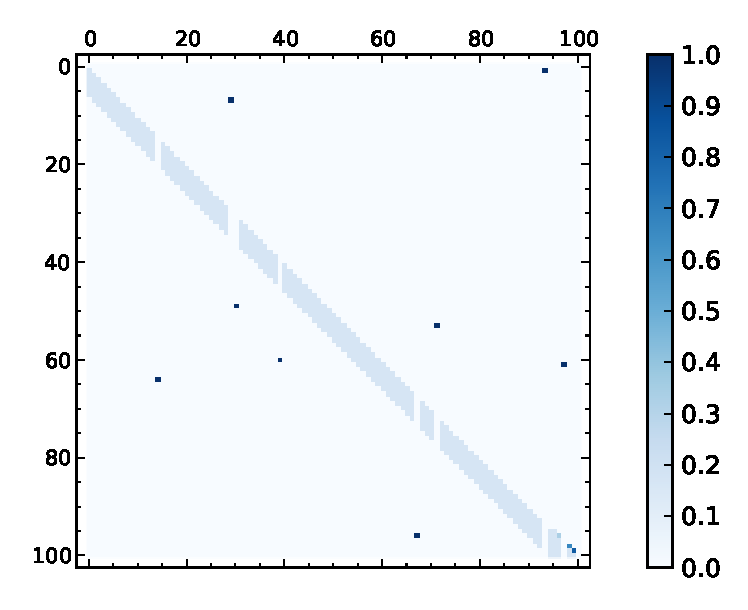
\includegraphics[scale=0.8]{images/matplot}
    \end{center}
  \end{figure}
\end{frame}

\begin{frame}{Results}
  \begin{figure}[!htbp]
    \centering
    \begin{subfigure}{.5\textwidth}
      \centering
      \includegraphics[width=\linewidth]{images/7plot}
      \caption{7 rolls}
    \end{subfigure}%
    \begin{subfigure}{.5\textwidth}
      \centering
      \includegraphics[width=\linewidth]{images/15plot}
      \caption{15 rolls.}
    \end{subfigure}
    \caption{The Probability Distributions after different numbers of rolls.}
  \end{figure}
\end{frame}

\begin{frame}{Results}
  \begin{figure}[!htbp]
    \centering
    \begin{subfigure}{.5\textwidth}
      \includegraphics[width=\linewidth]{images/turns}
      \caption{The Percentage of games that end ON turn $N$.}
    \end{subfigure}%
    \begin{subfigure}{.5\textwidth}
      \centering
      \includegraphics[width=\linewidth]{images/sumturns}
      \caption{The Percentage of games that end BY turn $N$.}
    \end{subfigure}
    \caption{Behaviour compared to $N$ rolls.}
  \end{figure}
\end{frame}

\begin{frame}{Contact Me}
  \begin{itemize}
    \itemsep2em
    \item Email: \href{mailto:campbellj11@cardiff.ac.uk}{campbellj11@cardiff.ac.uk}

    \item GitHub: \href{https://github.com/theref}{www.github.com/theref}

    \item LinkedIn
  \end{itemize}
\end{frame}

\end{document}
